\documentclass[11pt,twoside,fleqn]{scrreprt}
%\usepackage[utf8x]{inputenc}
%\usepackage[utf8]{inputenc}
\usepackage[T1]{fontenc}
%\usepackage[latin1]{inputenc}
\usepackage{graphicx}
\usepackage[margin=2.0cm,bottom=2.5cm]{geometry}
\usepackage{subfig}
%\usepackage{ulem}
\usepackage{fancyhdr}
\usepackage{hyperref}
\usepackage[usenames,dvipsnames]{color}
%\usepackage{amssymb}
\usepackage{amsmath}
%\usepackage{mathrsfs}
%\usepackage{textgreek}
%\usepackage{curves}
%\usepackage{latexsym} % ein paar Symbole
%\usepackage{textcomp} % ein paar Symbole
%\usepackage{natbib}
\usepackage{ulem}
\usepackage{bbm}
%\usepackage{mathtools}
%\usepackage{cancel}
%\usepackage{longtable}
%\usepackage{booktabs}
\usepackage[charter]{mathdesign}
%\usepackage{mathptmx}
\usepackage{url}
\usepackage{multicol}
\usepackage{authblk}
%\usepackage{nomencl}
\usepackage{makeidx}
\normalem

\nonfrenchspacing
\newcommand{\beq}{\begin{equation}}
\newcommand{\eeq}{\end{equation}}
\newcommand{\nn}{\nonumber}
\newcommand{\mwith}{\quad \mathrm{with} \quad}
\newcommand{\mand}{\quad \mathrm{and} \quad}
\newcommand{\mdiv}{\,\mathrm{div}\,}
\newcommand{\mDiv}{\,\mathrm{Div}\,}
\newcommand{\grad}{\,\mathrm{grad}\,}
\newcommand{\Grad}{\,\mathrm{Grad}\,}
\newcommand{\Cel}{\,$^\circ$C}
\newcommand{\dcdot}{\mbf{\,:\,}}
\newcommand{\tr}{\mathrm{tr}\,}
\newcommand{\mathd}{\mathrm{d}}
\newcommand{\mathD}{\mathrm{D}}
\newcommand{\mdiag}{\,\mathrm{diag\,}}
\newcommand{\mbf}[1]{\mbox{${\mbox{\boldmath${#1}$\unboldmath}}$}}
\newcommand{\mbfs}{\boldsymbol}
\newcommand{\dev}{\stackrel{def}{=}}
\newcommand{\tbf}{\textbf}
\newcommand{\tit}{\textit}
\newcommand{\mrm}{\mathrm}
%\newcommand{\citep}[1]{(\cite{#1})}
%\newcommand{\citet}{\cite}

\newcommand{\tf}{$\rightarrow\ $}
\newcommand{\ds}{\displaystyle}
\newcommand{\mtd}[2]{\frac{\mathd_{#1}{#2}}{\mathd t}} %material time derivative
\newcommand{\ptd}[1]{\frac{\partial {#1}}{\partial t}} %partial time derivative
\newcommand{\pd}[2]{\frac{\partial {#1}}{\partial {#2}}} %partial derivative
\newcommand{\vint}[1]{\int \limits_\Omega {#1} \mathd \Omega} %volume integral
\newcommand{\sint}[2]{\int \limits_{\partial \Omega_{#1}} {#2} \mathd \Gamma}
\newcommand{\uexp}[1]{$^{\mathrm{{#1}}}$}%superscript
\newcommand{\uind}[1]{$_{\mathrm{{#1}}}$}%subscript

\newcommand{\mvec}[1]{\uline{{#1}}}%Vektoren
\newcommand{\mmat}[1]{\uuline{{#1}}}%Matrizen

\newcommand{\drop}[1]{\red \cancelto{0}{\black #1} \black}

\newcommand{\centerpic}[3]{\hspace{#1\textwidth}\resizebox{#2\textwidth}{!}{\includegraphics{#3}}}





\setlength\parindent{0pt}%Festlegen des Absatzeinzuges
\setlength\parskip{10pt}%Festlegen des Absatzabstandes

\pagestyle{fancy}
\fancyfoot{}%clearall
\fancyhead{}%clearall
\renewcommand{\headrulewidth}{0pt} % no line in header area
\fancyfoot[LE,RO]{\thepage}           % page number in "outer" position of footer line
%\fancyfoot[RE,LO]{OGS6 -- Theory Manual} % other info in "inner" position of footer line

\makeindex

%\makenomenclature
%Define groups for nomenclature: Roman, Greek and Operators
%\RequirePackage{ifthen}
%\renewcommand{\nomgroup}[1]{\bigskip%
%\ifthenelse{\equal{#1}{R}}{\item[\textit{Roman symbols}]}{%
%\ifthenelse{\equal{#1}{G}}{\item[\textit{Greek symbols}]}{\ifthenelse{\equal{#1}{O}}{\item[\textit{Operators}]}}}}



\begin{document}
%List authors and affiliations here
\author[1]{Lars Bilke}
\author[1]{Thomas Fischer}
\author[1,2]{Olaf Kolditz}
\author[1]{Thomas Nagel}
\author[1]{Karsten Rink}
\author[1]{Agnes Sachse}
\author[1]{Haibing Shao}
\author[1]{Norihiro Watanabe}
\affil[1]{Department for Environmental Informatics, Helmholtz Centre for Environmental Research, UFZ, Leipzig, Germany}
\affil[2]{Environmental Systems Analysis, Dresden University of Technology, Dresden, Germany}
\makeatletter

%Generate titlepage
\date{\today}
\begin{titlepage}

\begin{flushright}

\includegraphics[height=0.1\textheight]{UFZ_logo}
\end{flushright}


\vspace{20mm}

\begin{center}
{\huge{OGS6 -- Theory Manual}}

\vfill
{\large{Document version: 0.1}}
\end{center}

\vspace{20mm}
{\large{Contributors:}}\footnote{In alphabetical order.}

{\large{
\@author}}

\end{titlepage}



\tableofcontents
\clearpage

%Nomenclature
%\printnomenclature%makeindex [].nlo -s nomencl.ist -o [].nls
%\nomenclature[gp]{$\phi_\alpha$}{Volume fraction of constituent $\alpha$.}
\nomenclature[gr]{$\rho_\alpha$}{Apparent density of constituent $\alpha$.}
\nomenclature[go]{$\mathd \Omega,\ \mathd \Omega_\alpha$}{Volume element of the mixture and constituent $\alpha$, respectively.}
\nomenclature[gr]{$\rho_{\alpha R}$}{Real density of constituent $\alpha$.}
\nomenclature[oh]{$\hat{(\bullet)}_\alpha$}{Production term of quantity $(\bullet)_\alpha$ due to local interaction with other constituents.}
\nomenclature[rv]{$\mbf{v}_\alpha$}{Velocity of phase $\alpha$.}
\nomenclature[od]{$\ds \mtd{\alpha}{(\bullet)}$, $(\bullet)'_\alpha$}{Material time derivative of $(\bullet)$ following the motion of phase $\alpha$.}
\nomenclature[od]{$\mdiv$}{Spatial divergence operator.}
\nomenclature[og]{$\grad$}{Spatial gradient operator.}
\nomenclature[rf]{$\mbf{F}_\alpha$}{Deformation gradient of phase $\alpha$.}
\nomenclature[rl]{$\mbf{l}_\alpha$}{Spatial velocity gradient of phase $\alpha$.}
\nomenclature[rj]{$J_\alpha$}{Determinant of the deformation gradient: $\det \mbf{F}_\alpha$.}
%\nomenclature[rq]{$q_R$}{Reaction rate.}
\nomenclature[rd]{$\mbf{D}$}{Diffusivity tensor.}
\nomenclature[gg]{$\mathd \Gamma$}{Area element.}
\nomenclature[rb]{$\mbf{b}_\alpha$}{External body force on phase $\alpha$.}
\nomenclature[rt]{$\mbf{t}_\alpha$}{Surface traction on phase $\alpha$.}
\nomenclature[rn]{$\mbf{n}$}{Outward unit normal vector.}
\nomenclature[rr]{$r_\alpha$}{Heat source/sink per unit mass associated with phase $\alpha$.}
\nomenclature[rq]{$\mbf{q}_\alpha$}{Heat flux vector associated with phase $\alpha$.}
\nomenclature[ru]{$u_\alpha$}{Specific inner energy of phase $\alpha$.}
\nomenclature[ge]{$\eta_\alpha$}{Specific entropy associated with phase $\alpha$.}
\nomenclature[rt]{$T_\alpha$}{Temperature of phase $\alpha$.}
\nomenclature[gp]{$\psi_\alpha$}{Specific Helmholtz free energy of phase $\alpha$.}
\nomenclature[oaa]{$\mbf{a} \cdot \mbf{b}$}{Dot product of $\mbf{a}$ and $\mbf{b}$.}
\nomenclature[oab]{$\mbf{A} \dcdot \mbf{B}$}{Double contraction of $\mbf{A}$ and $\mbf{B}$.}
\nomenclature[gm]{$\mu_\alpha$}{Gibbs free enthalpy.}
\nomenclature[gs]{$\mbfs{\sigma}_\alpha$}{Cauchy stress tensor of phase $\alpha$.}
\nomenclature[gse]{$\mbfs{\sigma}^E_\alpha$}{Cauchy extra stress tensor of phase $\alpha$.}
\nomenclature[gl]{$\mbfs{\lambda}_\alpha$}{Heat conductivity tensor of phase $\alpha$.}
%\nomenclature[rr]{$R_s$}{Specific gas constant.}
\nomenclature[rw]{$\mbf{w}_{\zeta}$}{Seepage velocity of constituent $\zeta$ relative to solid.}
\nomenclature[rw]{$\tilde{\mbf{w}}_{\zeta}$}{Filter velocity of constituent $\zeta$ relative to solid.}
\nomenclature[rk]{$\mbf{k}$}{Hydraulic permeability with units of [m$^\mathrm{4}$N$^\mathrm{-1}$s$^\mathrm{-1}$].}
\nomenclature[rks]{$\mbf{k}_S$}{Intrinsic permeability with units of [m$^\mathrm{2}$].}
\nomenclature[rcv]{$c_{\bar{v}}$}{Specific heat capacity at constant specific volume.}
\nomenclature[rcp]{$c_{p}$}{Specific heat capacity at constant pressure.}
\nomenclature[rv]{$\bar{v}$}{Specific volume.}
\nomenclature[rxm]{$x_{m\zeta}$}{Mass fraction of constituent $\zeta$ in gas phase.}
\nomenclature[rxn]{$x_{n\zeta}$}{Mole fraction of constituent $\zeta$ in gas phase.}
\nomenclature[rd]{$\mbf{d}_{\zeta}$}{Diffusion velocity of constituent $\zeta$ in gas phase.}
%\nomenclature[rp]{$\hat{\mbf{p}}_\alpha$}{Direct momentum production in phase $\alpha$.}
%\nomenclature[ge]{$\hat{\epsilon}_\alpha$}{Direct energy production in phase $\alpha$.}
\nomenclature[gmv]{$\mu_V$}{Viscosity of the gas.}
\nomenclature[rh]{$h_\alpha$}{Specific enthalpy.}
\nomenclature[rca]{$c_G$, $c_\zeta$}{Concentration of the gas or a gas component.}
\nomenclature[rda]{$\mbf{d}_{\alpha}$}{Rate of deformation tensor.}
\nomenclature[rn]{$n_\zeta$}{Number of moles of component $\zeta$.}
\nomenclature[rm]{$M_\zeta$}{Molar mass of component $\zeta$.}
\nomenclature[ri]{$\mbf{I}$}{Second order unity tensor.}
\nomenclature[rc]{$\mbf{C}_\alpha$}{Right Cauchy-Green tensor of phase $\alpha$.}
\nomenclature[ra]{$\mbf{a}_\alpha$}{Acceleration of phase $\alpha$.}
\nomenclature[od]{$(\bullet)^D$}{Deviatoric part of $(\bullet)$.}
\nomenclature[rf]{$\widetilde{\mbf{F}}_\alpha$}{Isochoric part of the deformation gradient.}
\nomenclature[rc]{$\widetilde{\mbf{C}}_\alpha$}{Isochoric part of the right Cauchy-Green tensor.}
\nomenclature[rr]{$R$}{Universal gas constant.}
\nomenclature[gb]{$\beta_p$}{Isothermal compressibility coefficient.}
\nomenclature[ga]{$\alpha_T$}{Isobaric thermal expansivity coefficient.}
\nomenclature[rna]{$N^a$; $\mbf{N}$}{Shape function of node a; vector/matrix of shape functions.}






%Introduction, User guide
\chapter{How to use this manual}

\section{What it is about}
This manual contains details of the theory behind OGS6. This encompasses both numerical as well as physical (process) issues. Process descriptions will contain specific assumptions, benchmark lists, governing PDEs and weak forms, linearisations where appropriate (Newton-Raphson) and FE matrices.

\section{Adding authors}
Anyone who adds content to this file should add their name and affiliation to the list in the main file at which point they will automatically appear on the title page. The format to include yourself is 
\begin{verbatim}
	\author[0815]{Smart McGenius}
	\affil[0815]{Gewandhaus Leipzig}
\end{verbatim}

\section{Adding content}
If you add content, create a subdirectory with an appropriate name (e.g. process type or name of the numerical algorithm) and use \texttt{input} in the main file to include your content.

\section{Nomenclature}
We ask authors to stick to the standard nomenclature provided as far as possible (i.e. not to define five different symbols for porosity) and add any new symbols to the nomenclature. To have all definitions in one place and facilitate maintainance please add nomenclature definitions to the file \textit{nomenclature.tex}

For example, the definition of a volume fraction $\phi_\alpha$ will be as follows
\begin{verbatim}
	\nomenclature[gp]{$\phi_\alpha$}{Volume fraction of constituent $\alpha$.}
\end{verbatim}
The first letter in the square brackets denotes which part of the nomenclature the defined symbol belongs to: \texttt{g} -- Greek symbols, \texttt{r} -- Roman symbols or \texttt{o} -- mathematical Operators. The second (and following) letter is used by Latex for alphabetic sorting.

\section{Keyword indexing}
If you refer to OGS keywords, please add them to the index by using the \texttt{\\kw} command. The first argument is reserved for special characters, usually a \texttt{\$} sign, and can be left empty for keywords without any special initial characters. The second argument is the keyword.
\begin{verbatim}
	The porosity is given by \kw{\$}{POROSITY}. 
\end{verbatim}
The command will ad the keyword without the leading special character to the index.

\section{References}
If you refer to published material reference it by including the appropriate *.bib file.

\section{Figures and labelling}
Figures should be provided as pdf or png files. Any labels given to figures and equations should be unique so as to avoid overlapping label definitions. We suggest to include a process acronym and author initials into the label to facilitate this, e.g.
\begin{verbatim}
	\label{eq:THM_NW_strain}
	\label{fig:GF_NB_layers}
\end{verbatim}

\section{Compilation}
The document is to be compiled with pdflatex:
\begin{verbatim}
	pdflatex Theory_Manual.tex
\end{verbatim}
The nomenclature can be built with
\begin{verbatim}
	makeindex Theory_Manual.nlo -s nomencl.ist -o Theory_Manual.nls
\end{verbatim}
The bibliography can be built with 
\begin{verbatim}
	bibtex Theory_Manual
\end{verbatim}
The index, finally, is built with:
\begin{verbatim}
	makeindex Theory_Manual
\end{verbatim}

\chapter{Reactive Transport Processes}

\section{Introduction to Reactive Transport Processes}

In the field of environmental and geosciences, the chemical components are often transported by fluids in porous or fractured media. During this process, if these components are having chemical reactions with each other, then we call it a reactive transport process. 

\subsection{Governing Equations}

Let $\mathbf{c}$ and $\mathbf{\overline{c}}$ be the concentration vectors of all mobile and immobile chemical components, and $f_{i}(\mathbf{c}, \mathbf{\overline{c}})$ represents the rate of consumption or production induced by the chemical reactions, the governing equations of reactive transport process can be written as, 

\begin{eqnarray}
\label{eqn:RT_react_trans}
\partial_{t} ( \theta \mathbf{c} ) + \bf{L} \mathbf{c} &=&  f_{i}(\mathbf{c}, \mathbf{\overline{c}}) \nonumber \\ 
\partial_{t} ( \theta \mathbf{\overline{c}} ) &=&  f_{i}(\mathbf{c}, \mathbf{\overline{c}}). 
\end{eqnarray}

\subsection{Available User Modules to simulate Reactive Transport Processes}

\begin{table}
\label{tab:RT_tab_rt_modules}
\caption{Reactive Transport User Modules implemented in ogs6. }
\begin{tabular}{c c p{5.5cm}}
\hline
Names of the User Modules    & Type of reactions & Underlying Numerical Algorithm \\
\hline
$\mathrm{REACT\_TRANS\_OPS}$      & Equilibrium and Kinetic Reactions    & Operator Splitting (Sequential Non-Iterative)      \\
$\mathrm{REACT\_GIA\_KIN}$        & Kinetic reactions only     & Global implicit approach with partial reduction scheme      \\
$\mathrm{REACT\_GIA}$            & Equilibrium and Kinetic Reactions     & Global implicit approach with reduction scheme      \\
\hline
\end{tabular}
\end{table}

Currently, there are three user modules implemented in ogs6 for the reactive transport simulations. Their names, underlying numerical algorithm, and applicable reaction types are summarized in Table ~\ref{RT_tab_rt_modules}. The difference between these two models is the underlying solution algorithm. For the operator splitting method, the left hand side of Equation \ref{eqn:RT_react_trans} is first solved. Then the concentration vectors on each finite element node are passed on to a chemical solver, the chemistry system on the right hand side is solved on one node after the other. For the global implicit method, the non-linear governing equations \ref{eqn:RT_react_trans} is solved in a monolithic way. The input files format for these two user modules are kept largely the same. 

The ogs5 users might know, that ogs5 adopted the operator splitting scheme to simulate reactive transport processes. Also, several different chemical solvers, like PhreeqC (CITATION), GEM (CITATION), and ChemApp (CITATION) have been integrated to run the nodal-based local chemistry systems. There are currently plans to re-implement these features into ogs6. Thus, the reactive transport user modules will be extended in the future. 

Here in this document, we focus on the two user modules $\mathrm{REACT\_TRANS\_OPS}$ \index{REACT_TRANS_OPS} and $\mathrm{REACT\_GIA}$\index{REACT_GIA}, since the $\mathrm{REACT\_GIA}$ module can also handle kinetic controlled reactions as well. 

\section{Setting up a Reactive Transport Process with ogs6}

\subsection{Project File Setting (*.PRO)}

One new file introduced since OGS6 is the project file (*.PRO). To demonstrate how this file is constructed, we are taking the benchmark case calcite as an example (see Fig. \ref{fig:RT_pro_file}). 

\begin{figure}
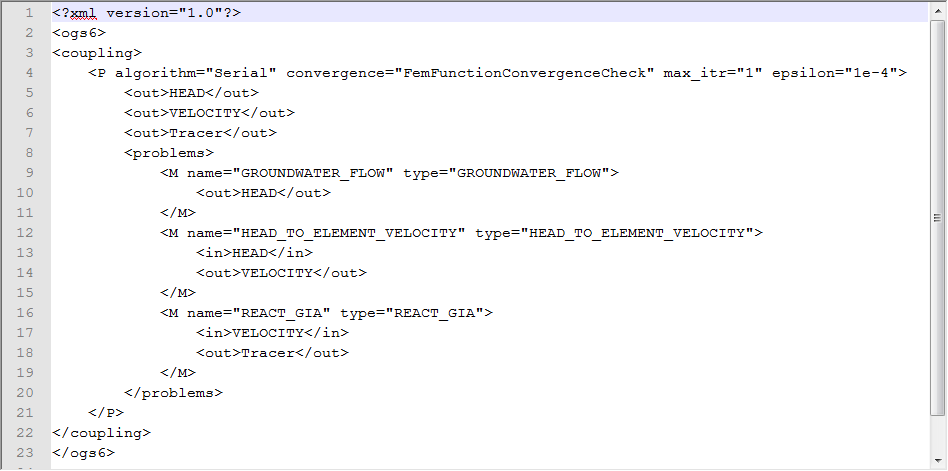
\includegraphics[width=\textwidth]{RT/figs/RT_fig_pro_file}
\caption{Example of project file definition for the benchmark case Calcite}
\label{fig:RT_pro_file}
\end{figure}

TODO: Explain the procedure

TODO: Explain possibilities of process interaction


\subsection{Geometry, Mesh, Media and Solid Properties (*.GLI, *.MSH, *.MMP and *.MSP)}

In OGS6, definition of geometry (*.GLI), mesh (*.MSH), media property (*.MMP) and solid property (*.MSP) are kept in the same format as in OGS5. Inside the OGS6 code, there is a conversion function to read the old file format and transfer the information into the new data structure in OGS6. To keep this tutorial concise, we would point the interested readers to the tutorial from Bauer et al (CITATION). It explains very well how these input files is defined. 

\subsection{Defining chemical Components (*.MCP)}

In the MCP file, we define the chemical components that will be involved in the chemical reactions. The general file format is kept the same as in ogs5. However, some changes are made to read in specific information. 

\subsubsection{MCP File Format}

\begin{figure}
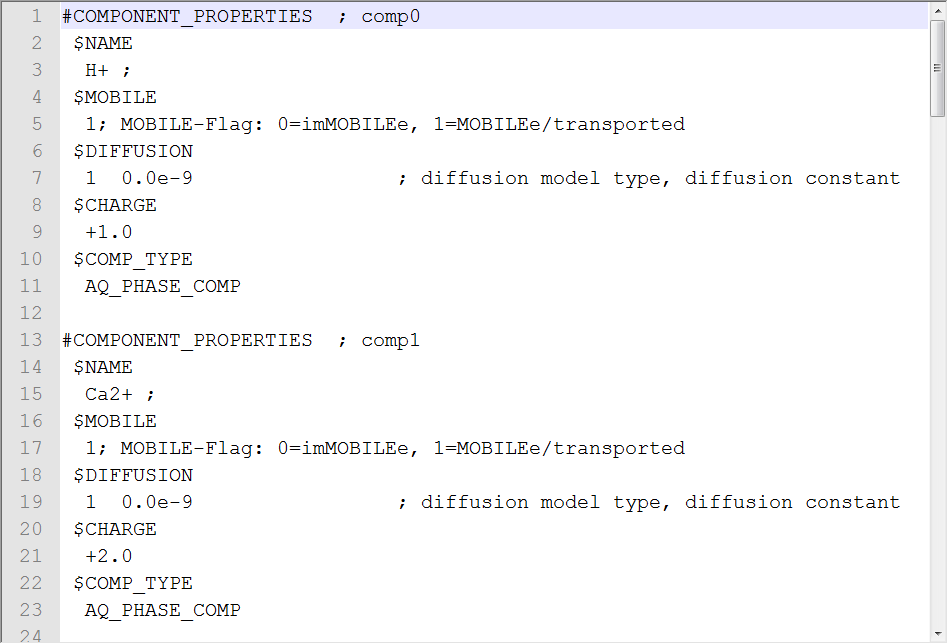
\includegraphics[width=\textwidth]{RT/figs/RT_fig_mcp_file}
\caption{Example of MCP file that is defining the chemical components in the calcite example.}
\label{fig:RT_mcp_file}
\end{figure}

As demonstrated in Fig. 2.2, we define the chemical components used in the reactive transport process. Each chemical components start with the key word $\#COMPONENT\_PROPERTIES$. In the calcite example, there are 5 key words used for each component. They are $\$NAME$, $\$MOBILE$, $\$DIFFUSION$, $\$CHARGE$, and $\$COMP\_TYPE$. As can be seen from the name of these key words, they are used to describe the name, mobility, diffusion model and coefficient, charge of the component, and type of the component. 

\subsubsection{Charge of Chemical Components}

The new features introduced in ogs6 are the last two key words, the $\$CHARGE$, and $\$COMP\_TYPE$. The $\$CHARGE$ key word will define how many equivalents of charge this chemical component is carrying with it. It is a double number, using the $+$ or $-$ sign to indicate the positive or negative charge. This key word is introduced, mainly because the charge information is needed to calculated the ionic strength of the solution, and thereafter needed in the activity coefficient correction. If no $\$CHARGE$ key word is defined in the MCP file, then the charge of corresponding component will be set to zero by default. 

\subsubsection{Types of Chemical Components}

\begin{table}
\label{tab:RT_tab_mcp_types}
\caption{Available types of chemical components and their meaning.}
\begin{tabular}{c p{5.5cm}}
\hline
$\$COMP\_TYPE$    & Meaning  \\
\hline
$BASIS\_COMP$       & Basis of the chemical reaction system (ref. section number) \\
$AQ\_PHASE\_COMP$    & Freely mobile component dissolved in the aqueous phase \\
$GAS\_PHASE\_COMP$   & Freely mobile component in the gas phase. \\
$MIN\_PHASE\_COMP$   & Single phase mineral component, its amount controlled by equilibrium mineral reactions.  \\
$SORPTION\_COMP$    & Sorption component that defined by a sorption reaction.  \\ 
$SS\_PHASE\_COMP$    & Solid Solution phase component (not yet fully supported) \\ 
$KIN\_COMP$         & Component, its amount solely controlled by kinetic reaction. \\
\hline
\end{tabular}
\end{table}

The $\$COMP\_TYPE$ key word reveals the type of the components. This is because the different types of chemical components, like aqueous phase components and mineral components, they are differently treated during the numerical simulation (ref. section number). It is very crucial to know this information, as some numerical scheme like $GIA\_REDUCT$ depends on it to make pre-and post-processing of the simulation. Currently, we have seven types built in OGS6, their names and differences are listed in Table \ref{tab:RT_tab_mcp_types}. 

The $\$KIN\_COMP$ type of component is quiet special. Actually, a mineral component can be defined as $\$KIN\_COMP$ type. Whether to define a mineral component to $\$MIN\_PHASE\_COMP$ or $\$KIN\_COMP$ depends on which type of reaction is controlling the amount of this mineral component. The former choice is exclusively attached to equilibrium mineral reaction, in which the present mineral is treated with activity of one. While the latter type is used only if this mineral is controlled by a kinetic rate expression. The reason of making this differentiation lies on the two separate numerical algorithms applied to simulate these two types of reactions. Interested readers please refer to section aa.bb for more details. For readers who would like to further work on the OGS development, please have a look into the source code: $\slash ogs6THMC \slash ChemLib \slash chemconst.h$.  One can find all types of components defined under the enum structure $Comp\_Type$. 


\subsection{Defining chemical Reactions (*.KRC)}

Once all the chemical components are ready in the MCP file, it is natural that the user would like to build their chemistry system by defining relevant reactions. We have adopted the old input file *.KRC file, which was used for kinetic reactions, and extended this file to accommodate both equilibrium and kinetic reactions. The advantage of this arrangement is that, old OGS5 input files can be easily supported by the new OGS6. However, we have to admit that it is a bit confusing when you see a equilibrium reaction defined under the same old key word $\#KIN\_REACT$. Figure 2.3 gives an illustration of how does the *.krc files looks like in the calcite example, which only contains equilibrium reactions. 

\begin{figure}
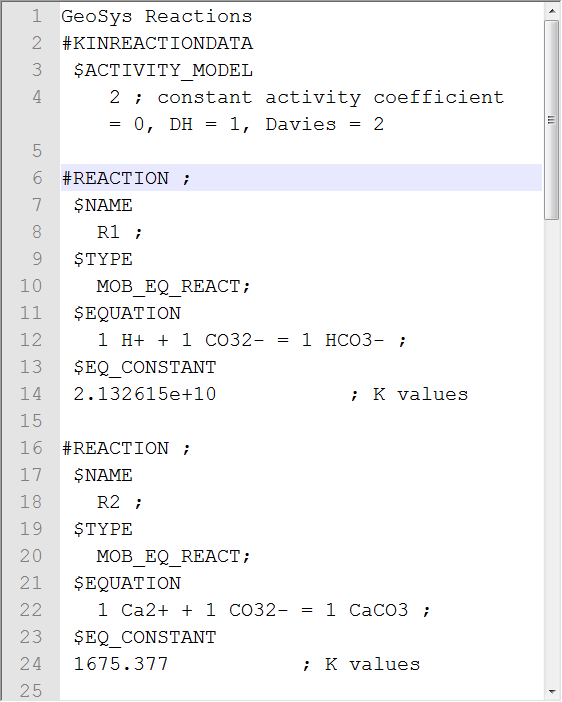
\includegraphics[width=0.5\textwidth]{RT/figs/RT_fig_krc_file}
\caption{Chemical Reactions definition file (*.KRC ) for the calcite example. }
\label{fig:RT_krc_file}
\end{figure}

\subsubsection{Equilibrium Reaction Definition}

As demonstrated in Fig \ref{fig:RT_krc_file}, the definition of an equilibrium reactions starts with the key word $\#REACTION$, and followed by key words like $\$NAME$, $\$TYPE$, $\$EQUATION$, and $\$EQ_CONSTANT$.  The name of the reaction in ogs6 does not have really influence on the simulation. It is merely adopted to differentiate different reactions. 

Currently, we have supported three types of equilibrium reactions, i.e. $MOB\_EQ\_REACT$, $SORP\_EQ\_REACT$, and $MIN\_EQ\_REACT$. From their names, it is easy to understand that for the $MOB\_EQ\_REACT$, all participating chemical components are mobile components dissolved in the aqueous phase. If this reaction is defining a sorption component or a single phase mineral component, then we use the corresponding key words respectively. 

One important issue to notice is the order of reactions. Conventionally, we start with the $MOB\_EQ\_REACT$, then the $SORP\_EQ\_REACT$ type, followed by the , and finished with the kinetic types of reactions. Well, in the future, there are already plans to automatically sort out these reactions during the pre-processing phase of the simulation. 

Under the key word \$EQUATION, the chemical reaction formula is given. As demonstrated in Figure \ref{fig:RT_krc_file}, for a chemical reaction 
$$ H^{+} + CO_3^{2-} \leftrightarrow HCO_3^{-} . $$
We write under the \$EQUATION key word the following text, 
$$ 1 ~ H+ ~ + ~ 1 ~ CO32- ~ = ~ 1 ~ HCO3- ~ . $$
Notice that, the strings ''H+'', ''CO32-'', and ''HCO3-'' are exactly the same as the component names defined in the MCP file. Before these component names, the number 1 reflects its stoichiometric ratiothat participates in the reaction. This number does not necessarily have to be a natural number, i.e. the user could also choose to define the same reaction by: 
$$ 0.5 ~ H+ ~ + ~ 0.5 ~ CO32- ~ = ~ 0.5 ~ HCO3- ~ , $$
although the corresponding equilibrium constant of the reaction must be changed accordingly. 

Another thing to be careful is the order of components. For a $MOB_EQ_REACT$, writing it with HCO3- as the reactant or the product does not change the reaction system, as far as the equilibrium constant is adjusted accordingly. However, defining a $MIN_EQ_REACT$ does require the mineral component to be written on the product side. For example, for the definition of calcite mineral precipitation and dissolution, we write the equation as, 
$$ 1 ~ CO32- ~ + ~ 1 ~ Ca2+ ~ = ~ 1 ~ Calcite; $$
The reason of this requirement is due to the complementary algorithm we have adopted in the code to handle mineral reactions. Interested readers please refer to section AA.BB for more detailed explanation. 
~\
To close the definition, the user needs to give out the equilibrium constant of the reaction, under the key word $\$EQ\_CONSTANT$.  Notice that in most of the thermodynamic databases, the equilibrium constant of a reaction is often given as in the log10 scale. The user needs to do a conversion of such values to linear scale. We have also provided another key word, $\$EQ\_CONSTANT\_LOG10$, under which the log10 scaled values can be directly used. 

\subsubsection{Kinetic Reaction Definition}

\begin{figure}
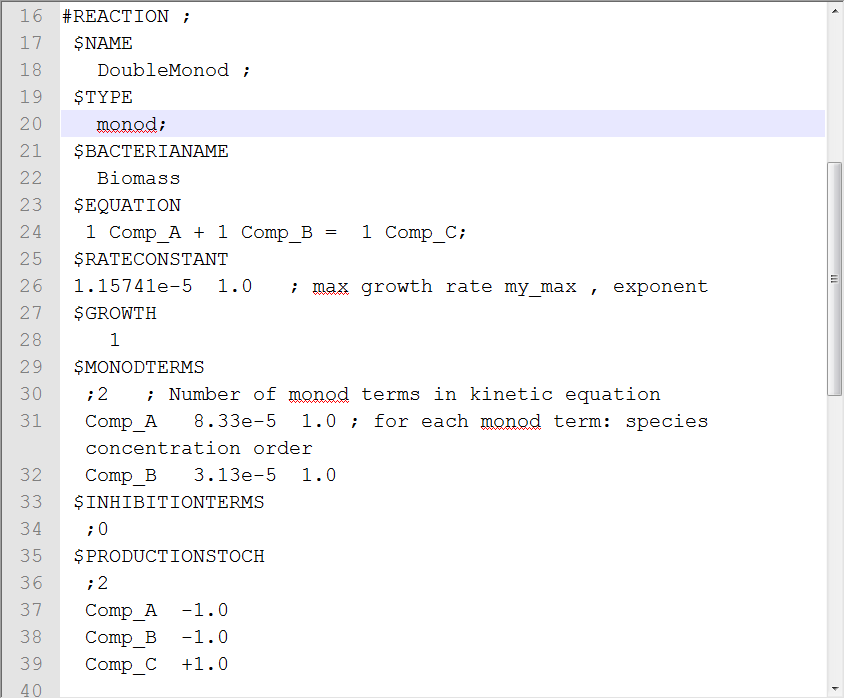
\includegraphics[width=0.5\textwidth]{RT/figs/RT_fig_monod_eq}
\caption{Demonstration of defining a monod type of kinetic reaction. }
\label{fig:RT_fig_monod_eq}
\end{figure}

The definition of a kinetic reaction is very similar as the equilibrium one. The definition also starts with the key word $\#REACTION$, followed by the name, type and equation of the reaction. So far there are only two types of kinetic reactions supported, i.e. the monod type and the user defined type $USER\_EXP$. 

In the application field of biochemical reaction, the monod type of kinetic reactions are often used. Such kind of reactions has a common rate expression as follows, 
\begin{equation}
rate = k^a \sum_{i=0}^{N} \left( \frac{C_i}{S_i + C_i} \right)^{n_i} \sum_{j=0}^{M} \left( \frac{I_j}{I_j + C_j} \right)^{m_i} 
\end{equation}

Let $N$ and $M$ be the number of monod growth and inhibition terms. $C_i$ and $C_j$ denotes the respective concentrations, $S_i$ and $I_j$ are the substrate concentrations of the monod and inhibition terms. $k$ refers to the reaction rate constant, with a the related exponential factor. $n$ and $m$ are the exponential factors for monod and inhibition terms. 

Figure \ref{fig:RT_fig_monod_eq} demonstrates the monod rate definition for the monod2d benchmark case. In this case, we have one growth term defined, which depends on the concentration of $Comp\_A$ and $Comp\_B$. The rate constant was set to 1.15741e-5, with the exponential factor of 1.0. The substrate concentration are 8.33e-5 and 3.13e-5 for $Comp\_A$ and $Comp\_B$ respectively. There are no inhibition terms involved. 

As we know from the experience, the rate expression of kinetic reactions can sometimes be very complicated, especially when the kinetic reactions are related to mineral or microbiological processes. We probably will never be able to include all types of kinetic rate expressions into the code, and most importantly, the user of the reactive transport code always would like to change these rate formulations to be adapted to their own applications. Therefore, we added a feature in our ogs6 code, that the user can define their own rate expression as they like. We take the reaction rate of dissolved organic carbon in the Neckar1D benchmark as an exmaple, its rate is regulated by the following expression, 
\begin{equation}
\frac{\partial C_{CH_2O}}{\partial t} = 1.57 \times 10^{-9} \times C_{CH_2O} \times \frac{C_{CH_2O}}{2.94 \times 10^{-4} + C_{CH_2O}}
\end{equation}
The user could actually write this expression in the KRC file.  Figure \ref{fig:RT_fig_user_exp} gives an example how the above rate expression can be defined. 

\begin{figure}
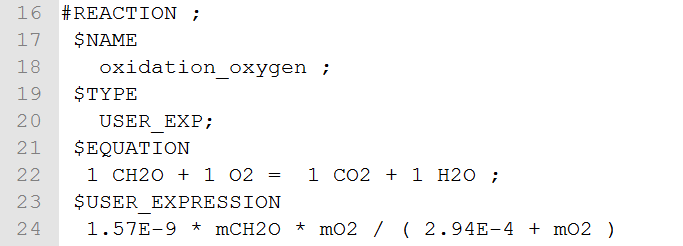
\includegraphics[width=0.6\textwidth]{RT/figs/RT_fig_user_exp}
\caption{Demonstration of user defined kinetic rate expression. }
\label{fig:RT_fig_user_exp}
\end{figure}

To use this feature, one need to first define the type of this kinetic reaction as $USER\_EXP$. Then under the key word $\$USER\_EXPRESSION$, the rate of the reaction can be formulated using the numerical number, mathematical operators (such as $+$, $-$, $*$, and $/$), logical operators, and brackets. In order to refer to the concentration of chemical component, the user needs to add a character ''m'' before the name of the chemical component. During the simulation, ogs6 will automatically obtain the mole concentrations (in the unit of mol$\slash$kg water) of corresponding component at particular node and apply them in user defined expression to calculate the rate values. 

This nice feature is achieved by the support of a external library called muParser \index{muParser}(\url{http://muparser.beltoforion.de}). The library is also an open-source project. Therefore we have included its source code directly into the ogs6. By the time when the kinetic reactions are initialized, we will also initialize the muParser library and defined the corresponding variables in the expression, such as the mole concentration of the chemical component. During the simulation, the evaluation function from the muParser library is called to give the rate values dynamically. The supported numerical and logically operations are actually defined by the muParser library. Interested readers are referred to their website for more details. 

When using the user defined rate expressions, one need to bear in mind that numerical operators like ''+'' and ''-'' can no longer be used as part of the chemical component name. For example, defining sulfate as ''SO42-'' is generally ok. But when the string ''mSO42-'' is referring to the concentration of sulfate in the rate expression, the muParser library is very likely to interpret the symbol as the subtraction operation, thus creating troubles. Our suggestion is, to avoid any operator symbols used as part of the component name. One may write ''SO42-'' and ''H+'' as ''SO4nn'' and ''Hp'', with the ''p'' and the ''n'' representing the positive and negative charge. Notice that we still have to give the charge as a numerical value under the $\$CHARGE$ key word (see section 2.4.2). 

The users need to keep in mind that, the evaluation of user defined rate expression is relatively slow compared to the built-in rate functions like monod. Therefore, when the rate expression is widely used, we recommend to implement it into the code and using it as a built-in function. 

\subsubsection{Activity Models}

In the OGS 6 code, we have provided support for the activity models. So far, the Debye-H\"uckel and Davies activity models (CITATION) have been implemented in OGS6. In the *.KRC file under the key word $\#KINREACTIONDATA$ and $\$ACTIVITY\_MODEL$, users will give an integer number to specify the activity model to be applied through the simulation (see Fig. \ref{fig:RT_krc_file}). Here ''0'' means activity coefficients are all set to unity. ''1'' refers to the Debye-H\"uckel model, and ''2'' stands for Davies model. If the key word $\$ACTIVITY\_MODEL$ is not given, then no activity model will be applied, this is then equivalent to the ''0'' case. 

\begin{figure}
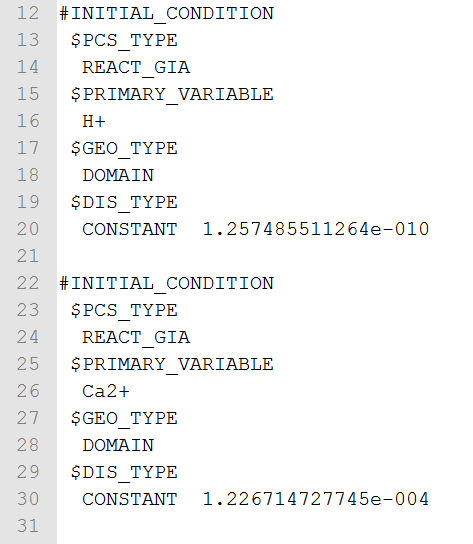
\includegraphics[width=0.6\textwidth]{RT/figs/RT_fig_ic_file}
\caption{Example of setting Initial Condition file (*.IC ) for the calcite example. }
\label{fig:RT_fig_ic_file}
\end{figure}

\subsection{Initial Conditions and Source/Sink Terms}

To construct a numerical model, initial and boundary conditions have to be specified by the user. Same as in OGS5, we write them in the *.IC, *.BC, and *.ST files. 

As in the reactive transport User Module, the primary variables are the concentrations of chemical components. Therefore, we define initial concentrations accordingly. Different components are specified under separate $\#INITIAL\_CONDITION$ key word. Fig. \ref{fig:RT_fig_ic_file} gives an illustration. Setting boundary conditions is very similar as setting initial conditions, except the key word $\#BOUNDARY\_CONDITION$ is used. 

\subsection{Time Stepping Settings}

\subsubsection{Fixed Time Stepping Scheme}

The fixed time stepping scheme is the most widely used time stepping setting. The user will need to specify the staring time, ending time, how many steps, and the size of each time step. Figure 2.7 demonstrate the format of *.TIM input files. In ogs6, the user will need to tell which UserModule the current time stepping scheme is applied to. Under the key word $\$TIME_STEPS$, the first number denotes the number of steps, and the second number is the size of each time step in the unit of seconds. The staring time and ending time of the simulation is specified under the key words $\$TIME_START$ and $\$TIME_END$. 

\begin{figure}
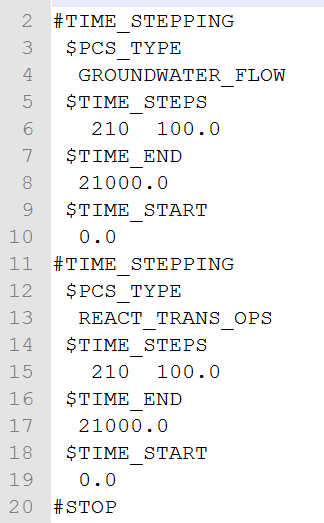
\includegraphics[width=0.5\textwidth]{RT/figs/RT_fig_fixed_tim}
\caption{Example of specifying fixed time stepping scheme. }
\label{fig:RT_fig_fixed_tim}
\end{figure}

In the configuration of Fig. \ref{fig:RT_fig_fixed_tim}, the User Module $GROUNDWATER\_FLOW$ is having the same time stepping scheme as the $REACT\_TRANS\_OPS$ module, i.e. 210 steps, each with 100 seconds. The user can also specify a gradually changing time step scheme. For example, we may want to run 10 steps first, with 10.0 seconds for each step, and then followed by 200 steps of 100.0 seconds each. The user can write ''10   10.0'' appending the key word $\$TIME\_STEPS$, followed by the ''200 100.0'' in the next line (demonstrated in Figure \ref{fig:RT_fig_adapt_tim}). 

\begin{figure}
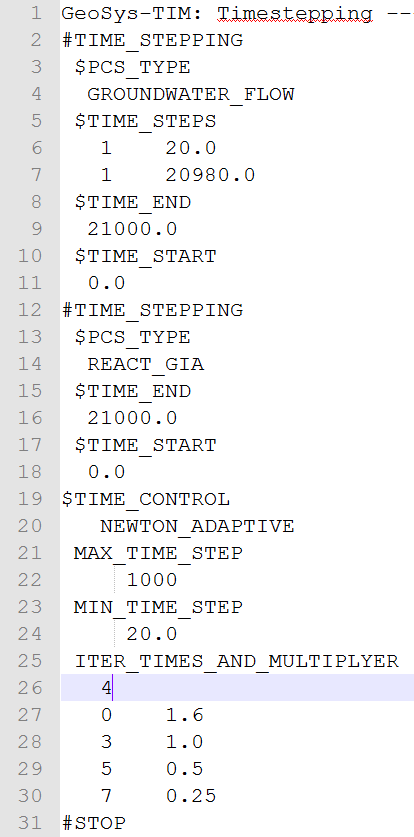
\includegraphics[width=0.5\textwidth]{RT/figs/RT_fig_adapt_tim}
\caption{Example of defining a Newton adaptive stepping scheme. }
\label{fig:RT_fig_adapt_tim}
\end{figure}

For different User Modules, they can also have unsynchronized time stepping scheme. For example, when we have a static groundwater flow model, the velocity field of groundwater will remain the same after the first time step. Therefore, we do not need to simulate the groundwater again if permeability remains unchanged. As demonstrated in Figure \ref{fig:RT_fig_adapt_tim}, the user can specify a very small time step for $GROUNDWATER\_FLOW$ and $REACT\_TRANS\_OPS$ process at the beginning. From the second time step on, $GROUNDWATER\_FLOW$ will not be simulated. In this case, the reactive transport process will automatically inherit the velocity field from the last time step.

\subsubsection{Adaptive Time Stepping Scheme}

When the UserModule $REACT\_GIA$ is applied, another choice provided is to use the adaptive time stepping scheme. The general principle is, the size of next time step, is dependent on the nonlinear Newton iterations from the previous time step. As demonstrated in Figure \ref{fig:RT_fig_adapt_tim}, the user needs to write $NEWTON\_ADAPTIVE$ under the key word $\$TIME\_CONTROL$.  Then, a series of threshold values have to be given under the key word $ITER\_TIMES\_AND\_MULTIPLYER$, to define the threshold regarding the number of Newton iterations and the multiplying factor for the next step. When one of the thresholds is achieved, the next time step size can be prolonged (e.g. multiplied by a factor of 1.6), kept the same (e.g. times a factor of 1.0) or shortened (e.g. by cut it into a quarter or half). From our experience, the best practice is to keep the number of Newton iterations between 2 to 4 times in each time step. The reason is, along with the growth of domain size, the time needed for assembling the Jacobian matrix and solving the linear equation system will grow exponentially. If we need more than 5 - 7 Newton iterations to converge the nonlinear problem, it is often more economic to cut the time step size and reduce the number of Newton iterations. Although it needs more steps to finish the simulation, the time needed altogether will still be shorter. 

\subsection{Numerical Settings(*.NUM)}

\begin{figure}
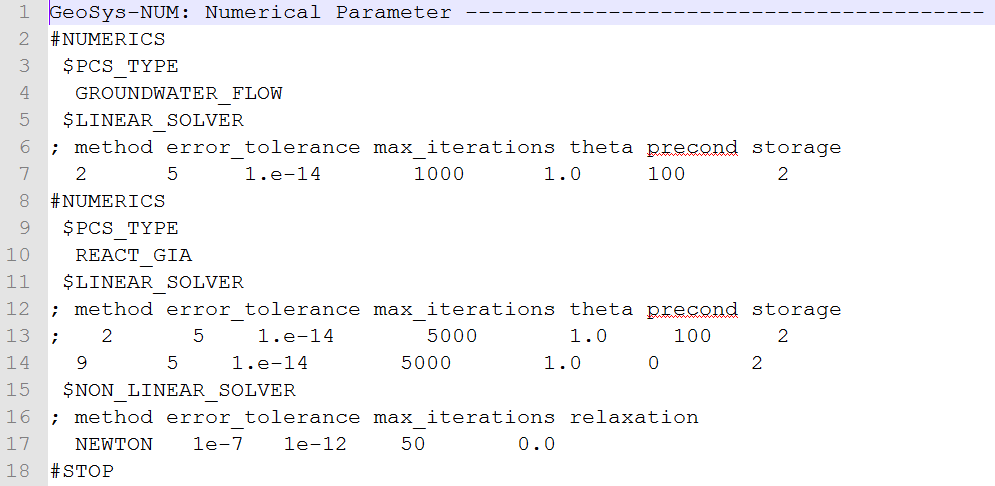
\includegraphics[width=0.9\textwidth]{RT/figs/RT_fig_num_file}
\caption{Example of numerical specification file. }
\label{fig:RT_fig_num_file}
\end{figure}

\begin{table}
\label{tab:RT_tab_linear_solvers}
\caption{Available types of linear solvers supported. }
\begin{tabular}{c p{5.5cm}}
\hline
Index    & Solver Types  \\
\hline
 1  & GAUSS \\
 2  & BICGSTAB \\
 3  & BICG \\
 5  & CG \\
805 & PARDISO \\ 
 9  & GMRES \\ 
\hline
\end{tabular}
\end{table}

In the *.NUM file, the numerical settings are specified for each user module. A typical NUM file is demonstrated in Figure 2.9. Under the key word $\$LINEAR\_SOLVER$, the method, error tolerance, max number of iterations, preconditoner methods are defined. Current supported linear solver method can be found in table \ref{tab:RT_tab_linear_solvers}. 

Under the key word $\$NON\_LINEAR\_SOLVER$, currently only the NEWTON method is supported by the reactive transport UserModule $REACT\_GIA$.  The tolerance, max number of iterations, and relaxation factor can be given accordingly. 


\subsection{Output Control(*.OUT)}

\begin{figure}
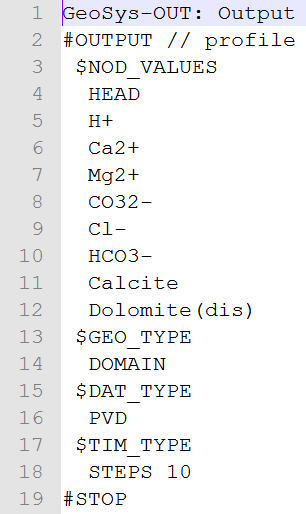
\includegraphics[width=0.3\textwidth]{RT/figs/RT_fig_out_file}
\caption{Example of numerical specification file. }
\label{fig:RT_fig_out_file}
\end{figure}

Before the simulation starts running, the user has to define in the *.OUT file, regarding which variables, and which time step the results should be plotted. Figure \ref{fig:RT_fig_out_file} shows the OUT file for the calcite example. Through the reactive transport process, the geochemical system is calculated on each node, internally there is a vector of concentrations for all chemical components. The user can then directly write the name of chemical components after the key word $\$NOD\_VALUES$. After the key word $\$GEO\_TYPE$, the user specify which geometry of the domain the result will be plotted. If the key word DOMAIN is given, then all nodal values will be plotted into the file. The key word $\$TIM\_TYPE$ defines the output time configuration. Key words STEPS 10 means that the results will be printed every 10 time steps. The user can also write explicitly in several subsequent lines the exact time that needs result output.   

\subsection{Running the Simulation}

\begin{figure}
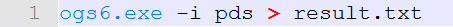
\includegraphics[width=0.5\textwidth]{RT/figs/RT_fig_bat_file}
\caption{A batch file example of running ogs6 simulation. }
\label{fig:RT_fig_bat_file}
\end{figure}

Running the simulation using ogs6 is a little bit different than ogs5. Originally, the user can double click ogs.exe file, and enter the path to the input files. For the new ogs6, we have to provide the path to input files, after a ''-i'' argument. So if typing it in the command line interface or call the ogs6 simulation inside a batch file, the command looks like Figure \ref{fig:RT_fig_bat_file}. Assuming the executable file ogs6.exe is residing in the same folder as the input files, the ''-i'' argument indicates that we are proving the input files pass. The string ''pds'' is the common name before different input file types. The ''$>$'' symbol tells the program that we would like to record all screen output in the result.txt file. 

\section{Common Errors and Pitfalls}

There are some very often encountered errors when using the ogs6 simulator. As developers, we are trying our best to prevent the user from entering unrealistic input information, which will drive the simulator into unproductive work. If the simulation is not working properly as you expected, the first thing the user shall look is the log file. That is why, we strongly recommend to store all screen output in an ASCII file like the result.txt. Now let’s have a look at several typical error messages that might appear in the log file, and analyze their reasons. 

\subsection{Missing Chemical Components}

\subsection{Errors in the reaction definition}

\subsection{Missing MMP/MSP definition}

\subsection{Handling negative Concentrations}



\section{Benchmarks Examples of Reactive Transport Processes}

\subsection{Decay1D with one kinetic reaction}

\subsection{Neckar1D with three kinetic reactions}

\subsection{Monod2D with kinetic reactions}

\subsection{calcite with Equilibrium Reactions}

\subsection{Calcite with mixed Equilibrium and Kinetic Reactions}

\renewcommand{\indexname}{Keyword index}
\printindex

\cleardoublepage
\bibliographystyle{plain}
\bibliography{common_bib_file}


\end{document}

